\documentclass[a4paper,4pt]{article}
\usepackage[a4paper, total={7in, 10in}]{geometry}
\setlength\parindent{0pt}
\usepackage[utf8]{inputenc}
\usepackage{graphicx} 
\usepackage{amsmath}
\usepackage{amsfonts}
\usepackage{amssymb}
\usepackage{listings}
\usepackage{ragged2e}
\usepackage{listings}
\usepackage{color}
\usepackage{pdfpages}
\usepackage[table]{xcolor}
\usepackage{soul}
\usepackage{siunitx}
\usepackage[hyphens]{url}
\usepackage{hyperref}
\usepackage{hyphenat}
\usepackage{multirow}
\usepackage{makecell}

\hypersetup{
    colorlinks=true,
    linkcolor=black,
    filecolor=magenta,      
    urlcolor=blue,
    pdftitle={Sharelatex Example},
    bookmarks=true,
    pdfpagemode=FullScreen,
    citecolor=black
}
% \setlength{\parskip}{\baselineskip}%
% \setlength{\parindent}{0pt}%
\begin{document}
\begin{titlepage}
	\centering
	
\includegraphics[width=.6\textwidth]{images/LiU_primary_black.png}\par
	\vfill
	{\scshape\Large \textbf{TDDE16}\par}
	{\huge\bfseries Extractive text summarization using TextRank Algorithm and text classification of news articles.\par}
	\vspace{0.75cm}
    {\large Lawrence Thanakumar Rajappa} \par
    {\large IDA Linköping University} \par
    {\large lawra776@student.liu.se}
	\vfill
	{\large \today\par}
\end{titlepage}
\renewcommand*\contentsname{Table of Contents}
\tableofcontents
\newpage
\listoffigures
\listoftables
\pagenumbering{gobble}
\newpage
\newpage
\clearpage
\pagenumbering{arabic}
\section{Abstract}
In this paper, I propose a system to summarize a news article using one of the Extractive Summarization techniques and 
classify the summarized news article using the deep learning model. To train and test, the data set used are news articles obtained
from British Broadcasting Corporation News (BBC News) \cite{greene06icml} which have been annotated by five classes: business, 
entertainment, politics, sports, and technology. The proposed framework uses the TextRank algorithm to summarize news articles
and a deep learning classification model is applied to classify them into classes mentioned above. Text summarizer combined 
with text classification helps many people such as academicians, politicians, business personnel, and etc. to read a large
chunk of text in a shorter period of time. Moreover, they could even use the classes to filter the summarized news to ease
their reading experience. In order to view the real working of these 2 models, news articles from both CNN News and 
BBC News channels are web scraped, summarized, classified and presented to the user through a web application.

\section{Introduction}
In the present era, we are dealing with information explosion everyday through various sources such as social network, IoT devices, government agencies, and etc. Hence,
we need a system to extract meaningful information faster and efficiently from those data. Automatic Text Summarization is one of 
the Text Mining techniques is used to identify important information in a document or a set of documents. It reduces the large texts to 
a considerable number of smaller sentences but preserving the overall meaning. This technique reduces the time taken to read large 
documents and helps to reduce the space required to store large documents. \par
\vspace{0.5cm}
In Automatic Text summarization, there exist two approaches 1) Abstractive Text Summarization, and 2) Extractive Text Summarization.
An extractive text summarization extracts important and meaningful sentences based on linguistic and statistical features \cite{gupta2010survey}. An
abstractive text summarization reads and understands an input file, generates the output with few words by identifying the main 
concept in the file \cite{madhuri2019extractive}. This document speaks about implementing extractive text summarization approach 
on news articles.

\subsection{Aim}
In this project, the aim is to create a system which will summarize the news articles from various sources such as BBC, CNN, NewYork
Times, and etc. using one of the extractive text summarization approaches - \textit{\textbf{TextRank Algorithm}} into smaller texts
and these summarized texts are classified into 5 different classes: business, entertainment, politics, sports, and technology 
using multiclass classification deep learning model. Later, these 2 models are used on the web scraped news articles from both CNN News and 
BBC News channels which are summarized, classified, and presented to the user through a web application.

\subsection{Motivation}
People across various fields such as politics, academics, business, and etc. need to know about the current happenings in the world 
using news articles. Hence, they either manually search for the news articles on the web or assign a person whose job 
is to gather news articles, summarize them manually, and present them in either paper-based or digital 
format \cite{businessPersonnel}. But, this process is time consuming and a huge workload. Moreover, some people make use of 
news monitoring tools available in the market to get the news by paying a monthly subscription fee \cite{newsmonitoring} which is not cost effective.
This project would solve the above-mentioned bottlenecks by creating a summarization system that could be used as a cost-free personalized service.
Additionally, in order to facilitate user's reading experience, the summarized texts are classified into 5 different classes to 
help people to read the texts by filtering them based on the area of interest.

\section{Related Work}
This section describes the methods that have been used in extractive text summarization and text classification. In the earlier researches, text
summarization on documents was done based on the proposed methods such as text summarization and classification using Capsule 
Networks and Sentence Embeddings \cite{LegoNet}, and 
topic modeling based text summarization \cite{topicmodelingSummarization}. \\
\par 
In 2020, Acharya et al. \cite{LegoNet} proposed a method for summarization and classification of Indian legal judgments.
The authors performed the proposed framework on 260 legal judgments created from two Indian legal data providers \textit{Manupatra,}
and \textit{Indian Kanoon}. Initially, documents are broken into sentences and sentence vectors for those sentences are extracted.
and classified into four types such as "fact", "argument", "judgment",
and "evidence" using Capsule Network architecture. Later, these sentence vectors are clustered using K-means algorithm \cite{macqueen1967some}. Sentences 
are selected which are closest to the centroid of each cluster based on a distance measure such as Euclidean Distance, 
Manhattan distance, and etc. and combined to form a coherent summary. \\
\par
In 2021, Roul \cite{topicmodelingSummarization} proposed a method for text summarization based on topic modeling. The 
author used different sets of Document Understanding Conferences data for this proposed framework. The proposed method 
finds the topic for each sentence in a document and sentence-topic matrix is generated where the entries are the importance 
of a topic T in a sentence S. Later, sentences are selected from each topic cluster and combined to form a summary.

\section{Theory}
In this section, concepts that are relevant to this project are going to be discussed. It is important to understand them for further
reading.
\subsection{Deep learning}
Deep learning is a subfield of Machine Learning and broader area which consists of many definitions provided by recognized 
universities, institutions, professors, and organizations and they are as follows,
\begin{itemize}
    \item Deep learning is a form of machine learning that enables computers to learn from experience and understand the
    world in terms of a hierarchy of concepts \cite{goodfellow2016deep}.
    \item Deep learning is a subset of machine learning in which multi-layered neural networks—modeled to work like the human 
    brain—'learn' from large amounts of data. Within each layer of the neural network, deep learning algorithms perform 
    calculations and make predictions repeatedly, progressively 'learning' and gradually improving the accuracy of the outcome 
    over time \cite{ibmDeepLearning}.
    \item Deep Learning is a machine learning technique that constructs artificial neural networks to mimic the structure and 
    function of the human brain. In practice, deep learning, also known as deep structured learning or hierarchical learning, 
    uses a large number hidden layers -typically more than 6 but often much higher - of nonlinear processing to extract features 
    from data and transform the data into different levels of abstraction (representations) \cite{deepAiDeepLearning}.
    \item and etc.
\end{itemize}
Artificial Neural Networks is the backbone for deep learning. An artificial neural network represents the structure of a human 
brain modeled on the computer. It consists of neurons and synapses organized into layers \cite{ann}.

\subsection{Word Embeddings}
Word embeddings are texts converted into numbers or vectors format. There may be different numerical representations for the 
same text and we convert texts to numbers because machines cannot understand texts like humans \cite{nss}. For any text based tasks, we 
need to convert every input text to vectors or numbers, which might be a time consuming. Hence, we could use a pre-trained 
word vectors such as GloVe, Word2Vec, ELMO, and etc. which are trained on large documents and consists of all word representations
which could increase the overall performance of our tasks and yield better results. An example of word representation is given below
for easier understanding. \\ \par
Consider the sentence "Text Summarization is a useful process". Here we break the sentence into list of words = ['Text','Summarization',
'is','a','useful','process']. The vector representation for the word 'Summarization' from the above list is [0,1,0,0,0,0], here the word 'summarization'
is replaced with 1 and other words are replaced by 0. Likewise, the vector representation for the word 'useful' from the above list is [0,0,0,0,1,0], here
for the word 'useful' is replaced by 1 and other words are replaced by 0. This is a simple word representation. In this project, we are
using GloVe word representation as the word embedding to perform text summarization.

\subsection{Term Frequency - Inverse Document Frequency (TF-IDF)}
\subsubsection{Term Frequency}
Term Frequency is defined as the number of times a term \textit{t} occurs in a document \textit{d} is called as Term Frequency of 
\textit{t} in \textit{d} and denoted by tf(\textit{t,d}) \cite{tfidf}. The formula for term frequency is illustrated in Figure \ref{fig:tf}.
\begin{figure}[h]
    \centering
    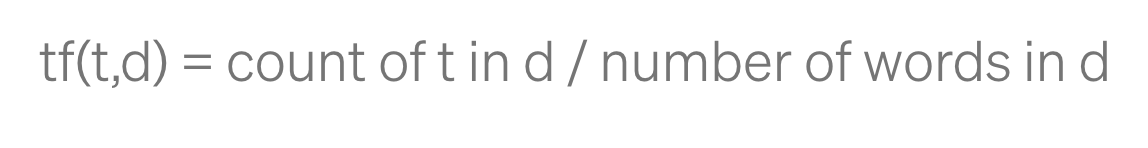
\includegraphics[scale=0.45]{images/tf.png}
    \caption{Term Frequency}
    \label{fig:tf}
\end{figure}
As the documents can be of varying length, it is possible for a term that would appear more frequently in longer documents than a 
shorter ones. As a result, it seems like a term would be more important to the longer document than to a shorter one. To redcuce this
problem, term frequency is often divided by the total number of terms in a document for normalization.

\subsubsection{Inverse Document Frequency}
Inverse Document Frequency is defined as the multiplicative inverse of document frequency (number of documents that contain a term \textit{t},
denoted by df(\textit{t}) \cite{tfidf}. Inverse Document Frequency is denoted by idf(\textit{t}).The formula for Inverse Document Frequency 
is illustrated in Figure \ref{fig:idf}.
\begin{figure}[h]
    \centering
    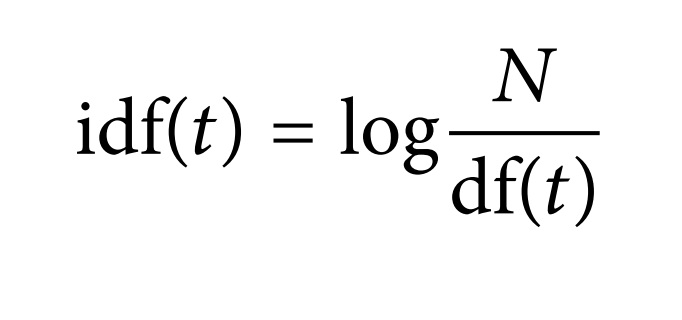
\includegraphics[scale=0.32]{images/idf.png}
    \caption{Inverse Document Frequency}
    \label{fig:idf}
\end{figure}

Where N denotes the number of documents. \\ \par

So combining Term Frequency and Inverse Document Frequency, provides more weightage to a word that occur frequently in a document
and in all other documents, while words that occur rarely are given lower weightage such that importance of words could be preserved \cite{tfidf}.
Higher the term weightage, the term is very much relevant to the document.
The formula for Term Frequency - Inverse Document Frequency is illustrated in Figure \ref{fig:tfidf}.
\begin{figure}[h]
    \centering
    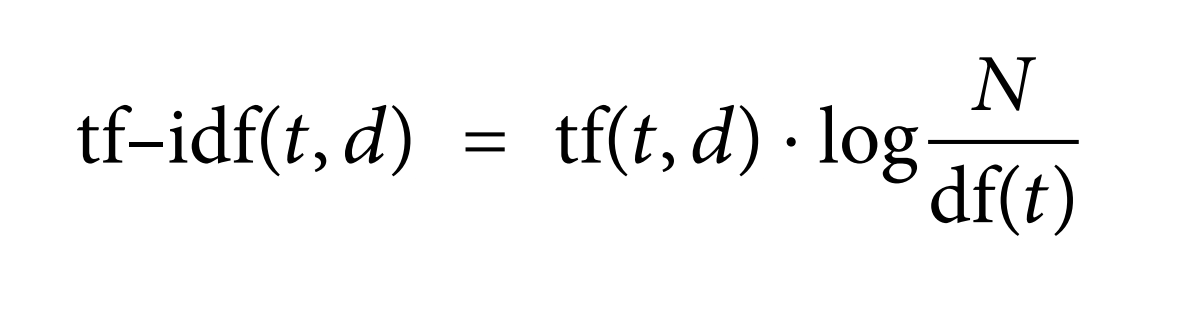
\includegraphics[scale=0.32]{images/tfidf.png}
    \caption{Term Frequency - Inverse Document Frequency (TF-IDF)}
    \label{fig:tfidf}
\end{figure}
\\
Where N denotes the number of documents.

\subsection{TextRank Algorithm}
TextRank is an extractive and unsupervised graph-based approach used in text summarization to generate document summaries \cite{textrank}.
TextRank algorithm is based on another algorithm known as \textit{PageRank Algorithm}. PageRank algorithm is used to rank web pages.
The rank is decided by the quality and number of links available in a web page. \\ \par 
The working of TextRank algorithm is given below,
\begin{itemize}
    \item Extract all sentences from the given text.
    \item A graph is created for the sentences. Nodes in the graph represent sentences while edges between two nodes represent weightage which
    is calculated by using a similarity function such as Cosine similarity, Jaccard similarity, and etc.
    \item Importance of nodes (scores) are found for each node by iterating the PageRank algorithm until convergence.
    \item The sentences are sorted in the descending order based on the score generated. The first \textit{n} sentences are selected
    to be part of the summary, where \textit{n} is the number of sentences.
\end{itemize}

\section{Data}
\subsection{Source of data}
The data used for both text summarization and text classification tasks are news articles obtained from British Broadcasting Corporation News 
(BBC News) which were used by Greene and Cunningham in their work - Kernel Document Clustering \cite{greene06icml}. The documents 
were provided as text files (.txt) for each news category such as business, entertainment, politics, sports, and technology.
\subsection{Structure of data}
The data consisted of 2225 documents of news articles along with their gold-standard summaries for the period 2004-2005 under 5 different news categories such 
as business, entertainment, politics, sports, and technology.
\subsection{Pre-processing of data}
The pre-processing process consists of following steps;
\begin{itemize}
    \item  The given input sentences are tokenized to get tokens of the terms.
    \item  The tokens are converted to lowercase.
    \item  The tokens are expanded if they are shortened by dropping a letter and replaced them by an apostrophe such as hadn't,
    hasn't, isn't, and etc.
    \item  The punctuations are removed from tokens.
    \item  The tokens are checked if they contain only alphabets or not.
    \item  Stopwords are removed from the list of tokens.
    \item  Finally, the tokens are merged together by a space literal and sent as an output.
\end{itemize}
The above pre-processing steps are same for both text summarization and text classification tasks.
\section{Methodology}
This section describes the framework used for text summarization and text classification. The proposed framework consists of 
1 function or a method for performing extractive text summarization and 1 deep learning model to classify the summarized text 
into 5 different categories such as business, entertainment, politics, sports, and technology. Initially, the user gets the news
articles based on the date range, geographical area, and etc. Later, these news articles are fed into the summarizer system and 
the ouput of the summarizer system is provided as an output to the news classifier model. Finally, the output of summarizer 
system and the output of news classifier model is displayed to the user through a web application. This proposed framework is
time efficient, environmental friendly (less paperwork) and user friendly. \\
\par
Section \textbf{6.1} describes the libraries or functions used in the proposed framework. Section \textbf{6.2} descibes about the 
extractive text summarization using TextRank. Section \textbf{6.3} describes the deep learning model to classify summarized news 
articles. Finally, section \textbf{6.4} describes about the web application developed by incorporating both text summarization and 
text classification models for helping users to read the long news articles in a short period of time.

\subsection{Libraries}
The following Python programming packages or libraries have been used by the proposed framework for data pre-processing and model building,
\begin{itemize}
    \item NumPy for numerical computations.
    \item Pandas for data loading.
    \item NLTK and Spacy.
    \item MatplotLib and Seaborn for visualization.
    \item Sklearn for evaluation metrics.
    \item Pickle for loading and saving of data objects, mathematical model objects and etc.
    \item NetworkX for creating graphs to store sentences and weights.
    \item OS to load the file from folders.
    \item Tensorflow for building deep learning model.
\end{itemize}

\subsection{Text Summarization using TextRank}
The text summarization method using TextRank algorithm summarizes large news articles into shorter texts which is easy to read and understand.
The dataset used for this task is BBC News articles for the period 2004-2005. The news articles are pre-processed as described 
above (\textit{see section 5.3}). The pre-processed news articles are sentence tokenized i.e. larger texts are broken into sentences
and vectors are extracted for those sentence by using the GloVe word embeddings. A similarity matrix is built by calculating Cosine similarity
between sentence vectors. Later, this similarity matrix is converted into graph and PageRank algorithm is applied to this graph to generate
ranks or sentence weightages. These sentence weightages along with sentence tokenized news articles are sorted in descending order.
Based on the number of sentence provided by the user, those number of sentences are selected from the sorted list and combined
together to form a summary. 
\subsection{Classification of News Articles}
The news classifier deep learning model classifies summarized news articles into 5 different categories such as business, 
entertainment, politics, sports, and technology. The dataset used for this task is BBC News articles for the period 2004-2005.
The data consists of 2225 rows of news articles. The number of news articles for various news categories are given below
(\textit{see figure \ref{fig:newscategories}}).
\begin{center}
    \begin{figure}[h]
        \begin{minipage}{.5\textwidth}
            \centering
            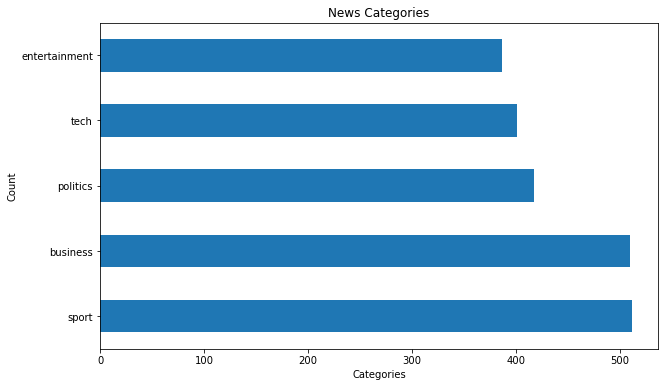
\includegraphics[scale=0.45]{images/categories_plot.png}
            \caption{Number of news articles in different news categories}
            \label{fig:newscategories}
        \end{minipage}
        \begin{minipage}{.6\textwidth}
            \centering
            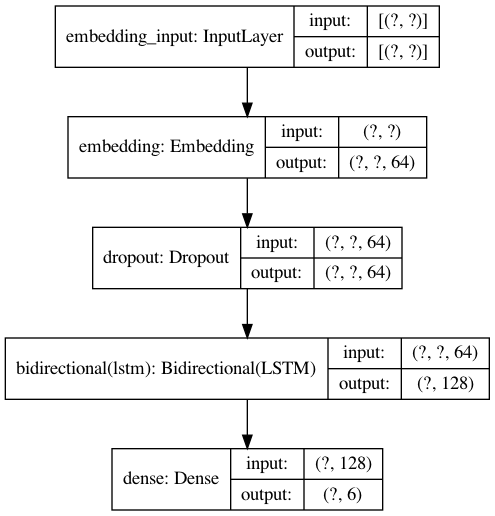
\includegraphics[scale=0.35]{images/model_plot.png}
            \caption{News Classifier Architecture}
            \label{fig:deeplearningarchitecture}
        \end{minipage}
    \end{figure} 
\end{center}
Initially, the given data is pre-processed (\textit{see section 5.3}) and split into training and test data where the training data 
size is 80\% and test data size is 20\%. A baseline model with Sklearn's dummy classifier is created under two different strategy 
$-$ stratified and most frequent. Baseline model with strategy as stratified only yielded 18\% as an accuracy on test data set, 
whereas baseline model with strategy as most frequent yielded 21\% as an accuracy on test data set.
But, after knowing the power of deep learning, a deep learning model is built and its architecture is given above (\textit{see figure \ref{fig:deeplearningarchitecture}}).
The pre-processed input is tokenized, sequenced and categories are label encoded i.e. a number is given for each news category are 
passed as an input to the above mentioned deep learning architecture and iterated for 10 epochs. 
At the 8\textsuperscript{th} epoch, the validation loss (0.1711) and training loss (0.0137) were very much less when compared with training and validation loss
values from other epochs. Hence, the model at 8\textsuperscript{th} epoch is saved for further use.
The output is a list of 5 probability values for each news categories from which highest probability value is selected and its 
index is matched against the indices of the news categories list which inturn is the respective category for the given input. \\
\par
The link to code repository for Text Summarization and Text Classification is \href{https://gitlab.liu.se/lawra776/extractive-text-summarization-and-classification-of-news-articles}
{https://gitlab.liu.se/lawra776/extractive-text-summarization-and-classification-of-news-articles}

\subsection{Text summarizer - a web application}
In order to put these 2 concepts for real-time use, a web-based application was created where these 2 functionalities are accessed 
through a REST API written in Flask. A user shall provide a \textit{from-date} and \textit{to-date} to read the summarized news 
article in that timeframe. The news articles are web scraped from the links (CNN and BBC) provided by \textit{MediaStack News API} 
using a python package called \textit{BeautifulSoup}. The news articles from both CNN and BBC are combined together and pre-processed.
These pre-processed news articles are summarized and classified and sent to the user as output where the user can filter the summarized
news articles based on the news classification. \\
\par The link to code repository for web application is \href{https://gitlab.liu.se/lawra776/news-summarizer}
{https://gitlab.liu.se/lawra776/news-summarizer} and link for screencast is given \href{https://liuonline-my.sharepoint.com/:v:/r/personal/lawra776_student_liu_se/Documents/Lawra776-TDDE16-web-application-screencast.mp4?csf=1&web=1&e=UuwHev}
{here}. \\
\par
The output of both the text summarization and text classification models will be dicussed in the forthcoming section.

\section{Evaluation Metrics}
In the field of deep learning there are several measures to know the quality and characteristics of a model. The most commonly used
evaluation metrics for classification task are \textit{Accuracy}, \textit{Recall}, \textit{Precision}, and \textit{F1 score}.
The evaluation metrics for text summarization task are \textit{ROUGE Scores}, \textit{BLEU Scores}, and \textit{Cosine similarity}. \\
\par
\textbf{Accuracy}: In general, the accuracy metric measures the ratio of correct predictions over the total
number of instances evaluated \cite{hossin2015review}, see \textit{figure \ref{fig:aprf}} for formula. \\
\textbf{Recall}: Recall is used to measure the fraction of positive patterns that are correctly classified \cite{hossin2015review}, 
see \textit{figure \ref{fig:aprf}} for formula. \\
\textbf{Precision}: Precision is used to measure the positive patterns that are correctly predicted from the total predicted 
patterns in a positive class \cite{hossin2015review}, see \textit{figure \ref{fig:aprf}} for formula. \\ 
\textbf{F1 Score}:This metric represents the harmonic mean between recall and precision values \cite{hossin2015review}, see \textit{figure 
\ref{fig:aprf}} for formula. \\
\textbf{ROUGE scores}: ROUGE stands for Recall-Oriented Understudy. It is a set of metrics for evaluating summarization of texts.
It compares a text summary generated by the algorithms or system summaries against a set of human-produced text summaries or 
gold standard summaries. A perfect match results scores to 1.0 and perfect mismatch results scores to 0. \\
\textbf{BLEU Scores}: BLEU stands for Bilingual Evaluation Understudy. It is a set of metrics for evaluating human-produced text summaries or gold standard  
summaries against candidate summaries or system summaries. A perfect match results scores to 1.0 and perfect mismatch results 
scores to 0. \\
\textbf{Cosine similarity}: Cosine similarity is one of the metric used to measure text similarity (it determines how two text documents
are close to each other in terms of their context or meaning) \cite{xia2015learning}, see \textit{figure 
\ref{fig:cosinesim}} for formula.
\begin{center}
    \begin{figure}[h]
        \begin{minipage}{.5\textwidth}
            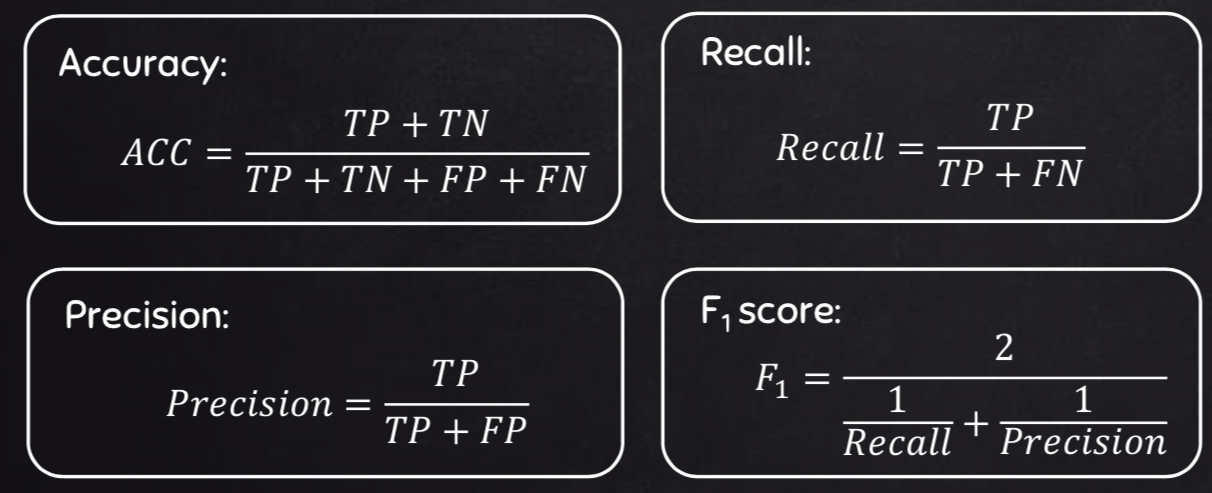
\includegraphics[scale=0.18]{images/evaluation_metrics_for_classification.png}
            \caption{Accuracy, Precision, Recall and F1 Score}
            \label{fig:aprf}
        \end{minipage}
        \begin{minipage}{.6\textwidth}
            \centering
            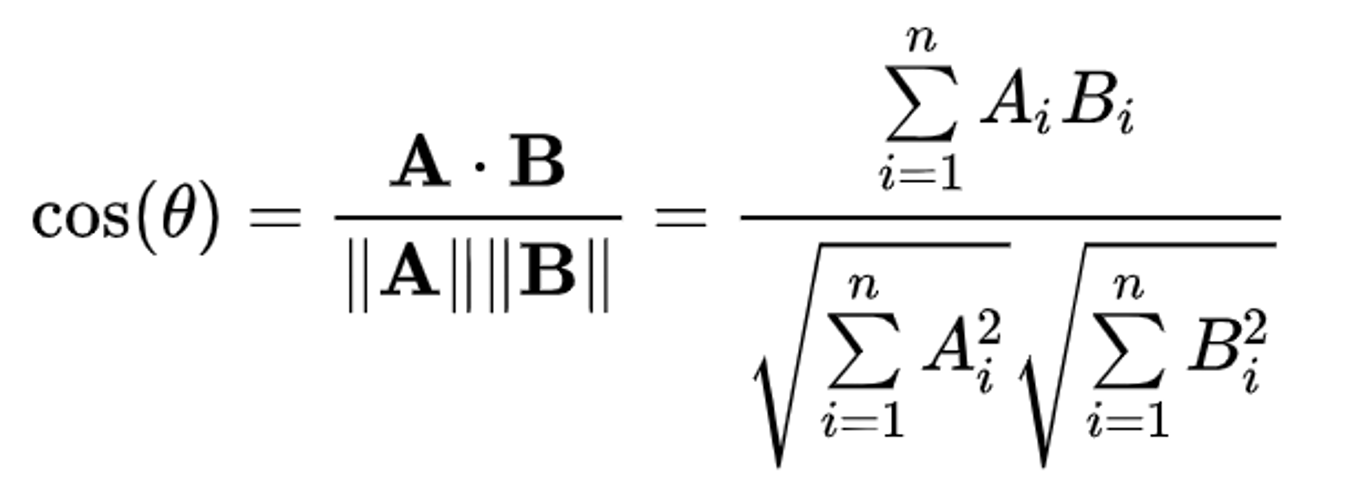
\includegraphics[scale=0.15]{images/cosine_similarity.png}
            \caption{Cosine Similarity}
            \label{fig:cosinesim}
        \end{minipage}
    \end{figure} 
\end{center}

\section{Results}
In this section, we will be seeing the results of text summarization and text classification models applied on the aforementioned
dataset (\textit{see section 5}). The outputs of two models are evaluated based on the metrics mentioned in \textit{section 7}.
\subsection{Text summarization evaluation}
By using the evaluation metrics for text summarization (\textit{see section 7}), the extractive text summarization function outputs 
are measured. Initially, a sample news article from the training data (1\textsuperscript{st} row) is used as an input for the function
to get the summarized news article. When cosine similarity is applied between summarized news article and the corresponding gold standard
summary, it yielded 0.92. Similarly, first 5 rows of news articles are pre-processed and sent as inputs to the text summarization function and 
the output is a list of summarized news articles. When ROUGE score (ROUGE-1 (unigram), ROUGE-2 (bigram), and ROUGE-L (long sequence)) 
and BLEU score calculated on the generated summaries with the gold standard summaries, it gave the following output. \\
\par
\begin{table}[h!]
    \parbox{.5\textwidth}
    {
        \begin{tabular}{|c|c|c|c|}
            \hline
            \multicolumn{4}{|c|}{ROUGE - 1} \\
            \hline
            \textbf{\makecell{News Article \\ No.}} & \textbf{Precision}& \textbf{Recall} & \textbf{F1-score} \\
            \hline
            1 & 0.63 & 0.30 & 0.40 \\
            \hline
            2 & 0.52 & 0.19 & 0.27 \\
            \hline
            3 & 0.73 & 0.18 & 0.29 \\
            \hline
            4 & 0.42 & 0.34 & 0.38 \\
            \hline
            5 & 0.27 & 0.42 & 0.31 \\
            \hline
        \end{tabular}
        \caption{ROUGE-1 scores for first 5 news article summaries}
        \label{table:rouge1}
    }
    \parbox{.5\textwidth}
    {
        \begin{tabular}{|c|c|c|c|}
            \hline
            \multicolumn{4}{|c|}{ROUGE - 2} \\
            \hline
            \textbf{\makecell{News Article \\ No.}} & \textbf{Precision}& \textbf{Recall} & \textbf{F1-score} \\
            \hline
            1 & 0.23 & 0.11 & 0.15 \\
            \hline
            2 & 0.19 & 0.07 & 0.1 \\ 
            \hline
            3 & 0.24 & 0.06 & 0.1 \\
            \hline
            4 & 0.16 & 0.13 & 0.38 \\
            \hline
            5 & 0.12 & 0.17 & 0.31 \\
            \hline
        \end{tabular}
        \caption{ROUGE-2 scores for first 5 news article summaries}
        \label{table:rouge2}
    }
\end{table}
\begin{table}[h!]
    \parbox{.5\textwidth}
    {
        \begin{tabular}{|c|c|c|c|}
            \hline
            \multicolumn{4}{|c|}{ROUGE - L} \\
            \hline
            \textbf{\makecell{News Article \\ No.}} & \textbf{Precision}& \textbf{Recall} & \textbf{F1-score} \\
            \hline
            1 & 0.70 & 0.39 & 0.50 \\
            \hline
            2 & 0.54 & 0.27 & 0.35 \\
            \hline
            3 & 0.73 & 0.26 & 0.39 \\
            \hline
            4 & 0.52 & 0.42 & 0.46 \\
            \hline
            5 & 0.34 & 0.39 & 0.36 \\
            \hline
        \end{tabular}
        \caption{ROUGE-L scores for first 5 news article summaries}
        \label{table:rougel}
    }
    \parbox{.4\textwidth}
    {
        \begin{tabular}{|c|c|}
            \hline
            \multicolumn{2}{|c|}{BLEU Score} \\
            \hline
            \textbf{\makecell{News Article \\ No.}} & \textbf{BLEU Score} \\
            \hline
            1 & 0.22 \\
            \hline
            2 & 0.21 \\ 
            \hline
            3 & 0.25 \\
            \hline
            4 & 0.21 \\
            \hline
            5 & 0.16 \\
            \hline
        \end{tabular}
        \caption{BLEU scores for first 5 news article summaries}
        \label{table:bleu}
    }
\end{table}

\subsection{Text classification evaluation}
By using the evaluation metrics for classification (\textit{see section 7}), the deep learning model attained a accuracy of 0.9989 on training data and 0.9506 on validation data
at 8\textsuperscript{th} epoch which are the best values when compared with other epochs. When the model was tested on the test 
dataset, it attained a F1 score of 0.951. The train and validation
data accuracy and loss at each epoch is given below (\textit{see figures \ref{fig:trainvalidacc} and \ref{fig:trainvalidloss}}).
\begin{center}
    \begin{figure}[h]
        \begin{minipage}{.5\textwidth}
            \centering
            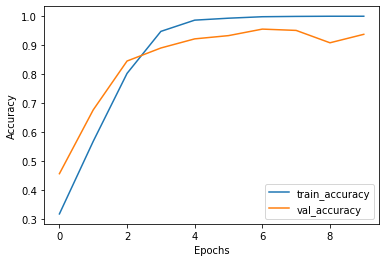
\includegraphics[scale=0.5]{images/text_classification_accuracy.png}
            \caption{Train-validation-data accuracy}
            \label{fig:trainvalidacc}
        \end{minipage}
        \begin{minipage}{.5\textwidth}
            \centering
            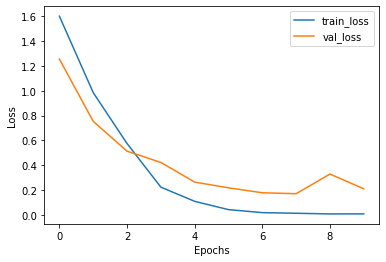
\includegraphics[scale=0.5]{images/text_classification_loss.png}
            \caption{Train-validation-data loss}
            \label{fig:trainvalidloss}
        \end{minipage}
    \end{figure} 
\end{center}
\begin{center}
    \begin{table}[h!]
        \centering
        \begin{tabular}{|c|c|c|c|c|}
            \hline
            \textbf{No. of epochs}& \textbf{Train-Accuracy} & \textbf{Validation-Accuracy} & \textbf{Train-Loss} & \textbf{Valid-Loss} \\
            \hline
            1 & 0.3174 & 0.4562 & 1.6007 & 1.2556 \\
            \hline
            2 & 0.5680 & 0.6764 & 0.9852 & 0.7537 \\
            \hline
            3 & 0.8022 & 0.8449 & 0.5754 & 0.5139 \\
            \hline
            4 & 0.9472 & 0.8899 & 0.2240 & 0.8899 \\
            \hline
            5 & 0.9860 & 0.9213 & 0.1096 & 0.2648 \\
            \hline
            6 & 0.9927 & 0.9326 & 0.0430 & 0.2185 \\
            \hline
            7 & 0.9978 & 0.9551 & 0.0188 & 0.1788 \\
            \hline
            \textbf{8} & \textbf{0.9989} & \textbf{0.9506} & \textbf{0.0137} & \textbf{0.1711} \\
            \hline
            9 & 0.9994 & 0.9079 & 0.0084 & 0.3296 \\
            \hline
            10 & 0.9994 & 0.9371 & 0.0087 & 0.2106 \\
            \hline
        \end{tabular}
        \caption{Train-validation data accuracy and loss at each epoch}
        \label{table:epochtable}
    \end{table}
\end{center}
\newpage
\section{Discussion}
In this section, we will be dicussing about the evaluated results of text summarization and text classification mentioned in
\textit{section 8}. \\ \par
From the values in the tables \ref{table:rouge1}, 
\ref{table:rouge2}, \ref{table:rougel}, and \ref{table:bleu}, it can be seen that the text summarizer
system is providing an average performance i.e. precision and recall score for ROUGE-1(unigram), ROUGE-2(bigram) and ROUGE-L(long sequence of text) are 
found to be in the range between 0.18 to 0.75 which states that 18\% to 75\% unigrams, bigrams and n-grams in the generated summary are also
present in the gold standard summary and BLEU score is in the range between 0.16 to 0.22 which also states that a system generated summary
sentences are also present in a gold standard summary and it can also be stated that generated summaries are a partial match with the 
gold standard summaries. \\
\par
From the table \ref{table:epochtable}, and figures \ref{fig:trainvalidacc} and \ref{fig:trainvalidloss}, it can be seen that 
news article classification deep learning model performs very well on training and validation data. 
Moreover, when this model tested on the test dataset and the yielded output when compared with gold standard news categories,
the F1 score, precision score and recall score for test data all equals to 0.95 or 95\% which once again proves that text 
classification model generalizes well on the unforeseen data.

\section{Conclusion}
In this paper, I proposed a system to summarize and classify a news article. A dataset with gold standard news categories
were obtained from BBC News along with their gold standard summaries was used to train a deep learning model. The system used the 
data to classify the news articles with an accuracy of 95\%. Later, the same data was used by the extractive text summarizer
to generate summary by selecting sentences from the news articles with higher score and combining them to form a coherent summary.
The generated summary is evaluated by using the ROUGE metric, BLEU metric and Cosine similarity.
The text summarizer combined with news articles classification model found to be an innovative approach for all people.
especially for reearchers, politicians, business personnel, and etc. as it would reduce the workload and time required to read through 
large chunk of text. 
\subsection{Further Improvements}
This approach could be further improved by performing any one of the following items;
\begin{itemize}
    \item The system could be improved by applying PoS tagging combined with dictionary rules on the corpus will improve 
    the sentence formation.
    \item Using ELMO and other word embeddings could help to preserve the context of a news article while it is being summarized.
    \item For faster response of the web-based system, big data tools such as Apache Spark, Apache MapReduce, and etc. could be used 
    to parallel process the documents to summarize and classify them.
\end{itemize}
\addcontentsline{toc}{section}{References}
\bibliographystyle{IEEEtran}
\bibliography{references}
\end{document}